\chapter{Implementation Overview}
\label{ch:developers_guide}
\label{ch:programmers_guide}

When we were creating our application, we kept in mind to make it as easy as possible for users to use. Therefore, we opt for a web-based interface with which users come in contact daily. From the user point of view, it does not require the installation of any additional application, and it can be used across many operating systems.

Creating a simple, shareable environment for users allows us to collect more annotated data. Compared to the classical applications, which need to be installed on each user's computer, a web-based application needs to be set up just on the server by the researcher and then users can simply access it by the web address. This way, it may be easier to reach a bigger audience.

For our back-end we decided to use Python, because it has a big machine learning community with ever-growing possibilities of open-source projects. As a result of this, we decided to use Django --- easily scalable Python web-framework.

Since our implementation covers a wide range of tasks --- from a web-based front-end to a library able to work with deep learning models, we do not include an exhaustive enumeration of the specific classes and functions in this chapter. Instead, we provide an overview of the individual parts of the application. We start with the separation of the application into three layers, as displayed in \autoref{fig:implementation_overview}.

This figure represents the individual layers of our framework and provides a summary of the technologies used. Our application consists of two main Python modules: \verb+diplomova_praca+ and \verb+diplomova_praca_lib+. In the figure, the front-end and back-end belong to the first one, and the library represents module \verb+diplomova_praca_lib+.

We shortly describe each of the layer, as displayed in the figure.

\section{Front-end}

Our front-end consists of several Django templates (a way to create HTML files dynamically), with the corresponding styling. We then use jQuery to provide a user with an interactive environment in the application.  The part of displaying the menu and the results are shared between both modules --- face and spatial. The interactive content --- canvas for the spatial and the grid for faces --- is dynamically added based on the currently selected module.

\subsubsection*{Design}
For a unified look, we follow the Material Design guidelines. We use some of the components from Material Design Lite. To complement the overall design, we also use Material Design Icons.

We style our own components with using the Cascading Style Sheets. We use Syntactically Awesome Style Sheets (commonly known as SCSS) to reduce the amount of code. One of the advantages of SCSS compared to CSS is the support of variables and nesting. We use this, for example, when setting the colors for the whole application. This way, we can provide users with a unified color scheme, while the colors can be easily adjusted for a different color scheme, if needed.

\subsubsection*{Interaction}

To provide a smooth user experience, without any unnecessary loading during the search, we use JavaScript. For some actions, like dragging, resizing we utilize functionalities from jQuery\footnote{\url{https://jquery.com/}}. 

To avoid reloadings, we update the content using JavaScript and we obtain the data via asynchronous communication with our Django back-end. One of the advantages of this approach is that the user can continue experimenting with the collage while the system is retrieving the results.

We do the communication with the Django as asynchronous HTTP POST requests. We encode the data as JSON, or directly as a string, if possible. The data are of different types; for example, in the spatial module, we need to send all images with their relative position. In the case of the face module, we include the Tree View, i.e., the current level and position in the layer.

\section{Back-end}

The goal of our back-end is to process the HTTP requests from front-end and transform them into Python objects. This way, we can directly query our library by calling the functions and passing the Python objects. The back-end also initializes the datasets in the library. Additional functionality of the back-end is the choice of the target image out of available images. Secondary functionalities include logging submitted collages and additional data into the database.

\section{Library}

In the library, we implement all approaches mentioned in this thesis. The library includes all the feature extraction methods, image handling, training, plots generation, and more.

Since the content of the library is broad, we separate it further into four main blocks: 
\begin{itemize}
    \item Annotation and Preprocessing --- scripts used for extraction of the features from a custom dataset
    \item \verb+face_features/+ -- face module, which is responsible for creating the multilevel structure (\verb+TreeView+). It also contains models for the extraction of faces and the face encodings.
    \item \verb+position_similarity/+ -- spatial module, which includes used models and the feature extraction techniques (as regions or antepenultime approach). The entry point for any request is function \verb+positional_request()+ in the file \verb+position_similarity_request.py+. We use this entry point also for our experiments.
    \item Additional scripts (\verb+helpers/+) -- this includes all the scripts to run and evaluate the experiments. These are not necessary for the application itself, but useful while investigating the approaches or the data.
\end{itemize}

\subsubsection*{Attribution}

At last, we would like to express our gratitude to the authors of all the used technologies provided by an open-source community. Additionally, to the projects mentioned in the text, we would like to thank the authors of crucial libraries such as Scikit-learn \citep{pedregosa2011scikit} and NumPy \citep{van2011numpy}.

\begin{figure}
    \centering
    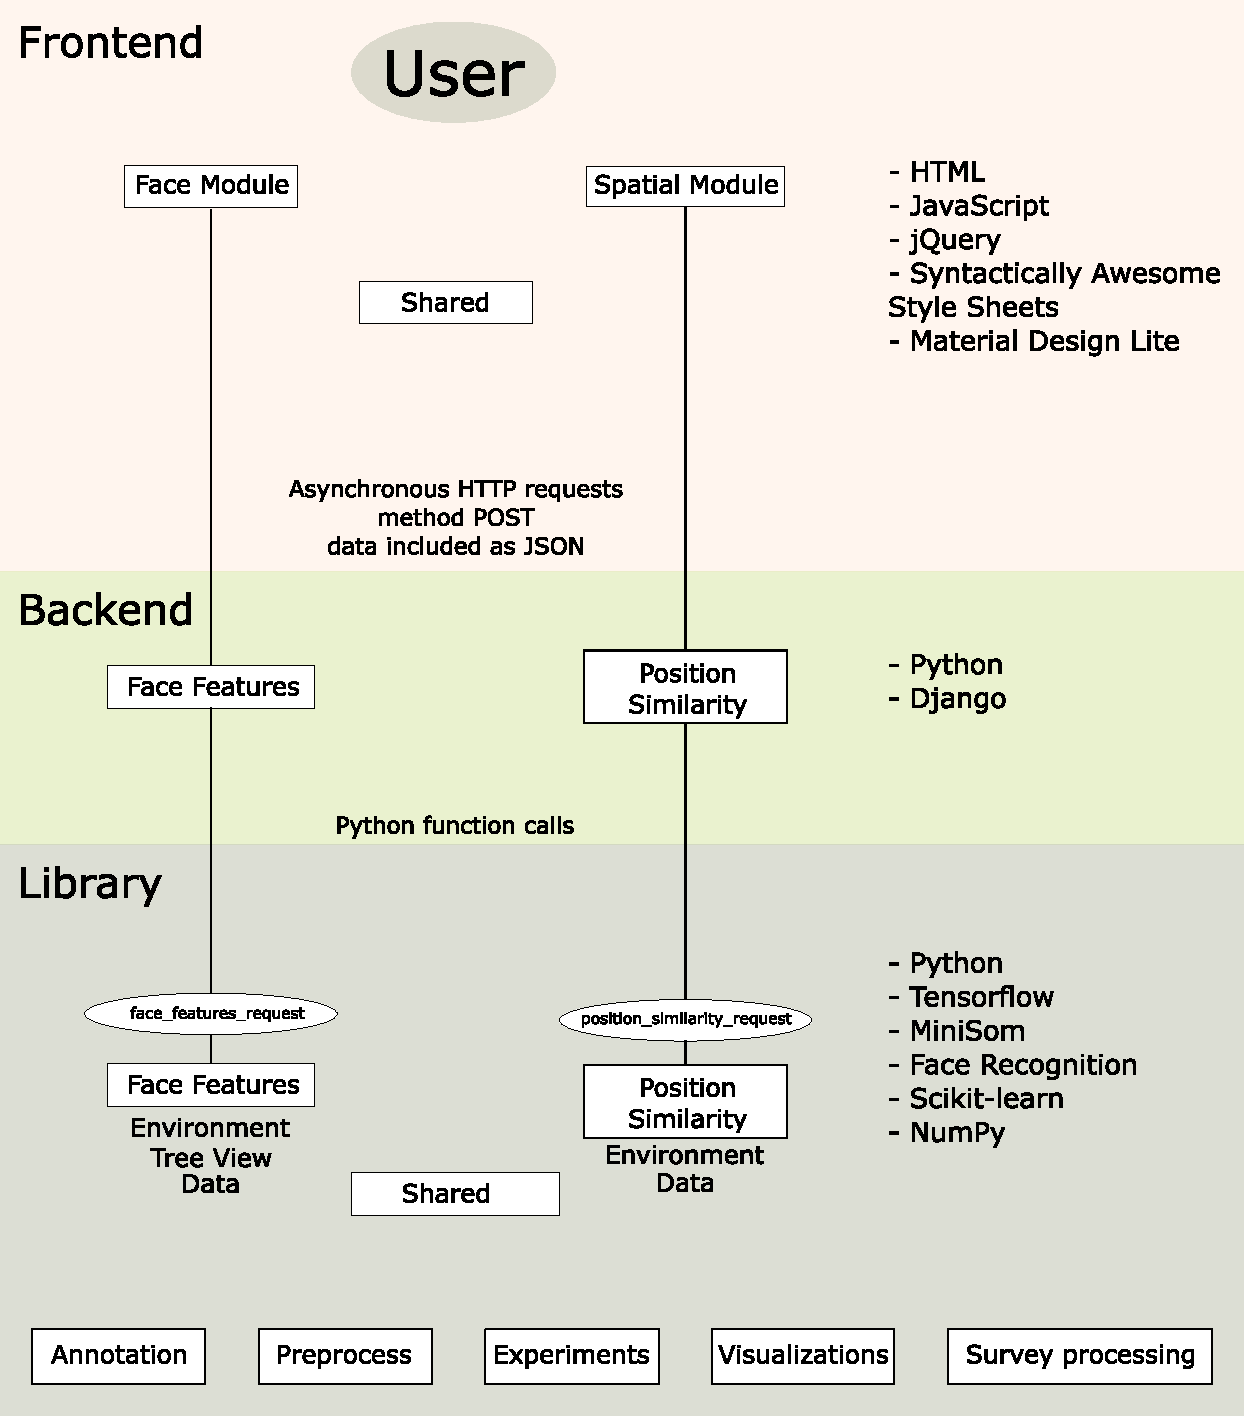
\includegraphics[width=0.95\linewidth]{graphs/implementation_overview.pdf}
    \caption{Overview of the implementation}
    \label{fig:implementation_overview}
\end{figure}